\documentclass[a4paper,12pt]{article}
\usepackage{amssymb}
\usepackage{amsmath}
\usepackage{amsthm} 
\usepackage{caption}
\usepackage{misccorr}
\usepackage[noadjust]{cite}
\usepackage{cmap} 
\usepackage[utf8]{inputenc}
\usepackage[T2A]{fontenc}
\usepackage[english, russian]{babel}
\usepackage{indentfirst}
\setlength{\parindent}{5ex}
\usepackage{graphics}
\usepackage{graphicx}
\usepackage{textcomp}
\usepackage{verbatim}
\usepackage{makeidx}
\usepackage{geometry}
\usepackage{float}
\usepackage{bm}
\usepackage{esint}
\usepackage{mathtools}
\usepackage{graphicx}
\usepackage{listings}
\usepackage{courier}
\usepackage{multirow}
\usepackage{graphicx}

\lstset{basicstyle=\fontsize{10}{10}\selectfont,breaklines=true}

\newcommand{\specchapter}[1]{\chapter*{#1}\addcontentsline{toc}{chapter}{#1}}
\newcommand{\specsection}[1]{\section*{#1}\addcontentsline{toc}{section}{#1}}
\newcommand{\specsubsection}[1]{\subsection*{#1}\addcontentsline{toc}{subsection}{#1}}
\newcommand{\RNumb}[1]{\uppercase\expandafter{\romannumeral #1\relax}}
\newcommand{\jj}{\righthyphenmin=20 \justifying}


% геометрия
\geometry{pdftex, left = 2cm, right = 2cm, top = 2.5cm, bottom = 2.5cm}

\setcounter{tocdepth}{4} % фикс переноса 
\righthyphenmin = 2
\tolerance = 2048

\begin{document}
\thispagestyle{empty}

\noindent \begin{minipage}{0.15\textwidth}
	
\includegraphics[width=\linewidth]{b_logo}
\end{minipage}
\noindent\begin{minipage}{0.9\textwidth}\centering
	\textbf{Министерство науки и высшего образования Российской Федерации}\\
	\textbf{Федеральное государственное бюджетное образовательное учреждение высшего образования}\\
	\textbf{«Московский государственный технический университет имени Н.Э.~Баумана}\\
	\textbf{(национальный исследовательский университет)»}\\
	\textbf{(МГТУ им. Н.Э.~Баумана)}
\end{minipage}

\noindent\rule{18cm}{3pt}
\newline\newline
\noindent ФАКУЛЬТЕТ $\underline{\text{«Информатика и системы управления»}}$ \newline\newline
\noindent КАФЕДРА $\underline{\text{«Программное обеспечение ЭВМ и информационные технологии»}}$\newline\newline\newline\newline\newline\newline\newline


\begin{center}
	\noindent\begin{minipage}{1.3\textwidth}\centering
	\Large\textbf{  Лабораторная работа № 5}\newline
	\textbf{по дисциплине "Вычислительные алгоритмы"}\newline\newline\newline
	\end{minipage}
\end{center}

\noindent\textbf{Тема} $\underline{\text{Построение и программная реализация алгоритмовчисленного интегрирования.}}$\newline\newline
\noindent\textbf{Студент} $\underline{\text{Мицевич М. Д.}}$\newline\newline
\noindent\textbf{Группа} $\underline{\text{ИУ7-41Б}}$\newline\newline
\noindent\textbf{Оценка (баллы)} $\underline{\text{~~~~~~~~~~~~~~~~~~~~~~~~~~~}}$\newline\newline
\noindent\textbf{Преподаватель} $\underline{\text{Градов В.М.}}$\newline

\begin{center}
	\vfill
	Москва~---~\the\year
~г.
\end{center}
\clearpage

\section{Цель работы}

\noindent Получение  навыков  построения  алгоритмавычисления  двукратного интеграла с использованием квадратурных формул Гаусса и Симпсона.

\section{Исходные данные}
\noindent Дан двукратный интеграл

\[\epsilon(\tau) = \frac{4}{\pi} \int_{0}^{\frac{\pi}{2}}d\phi\int_{0}^{\frac{\pi}{2}}[1 - 
exp(-\tau\frac{l}{R})]\cos(\theta)\sin(\theta)d\theta\]

\[\frac{l}{R} = \frac{2\cos{\theta}}{1 - \sin^2{\theta}\cos^2{\phi}}\]

\noindent Требуется применить  метод  последовательного  интегрирования.    По  одному  направлению использовать формулу Гаусса, а по другому - формулу Симпсона.

\section{Код программы}
\noindent\textbf{Листинг main.py:}
\lstinputlisting[frame=single, language=Python]{main.py}

\noindent\textbf{\newline Листинг gauss.py:}
\lstinputlisting[frame=single, language=Python]{gauss.py}

\noindent\textbf{\newline Листинг simpson.py:}
\lstinputlisting[frame=single, language=Python]{simpson.py}

\section{Результаты}
\subsection{Описать алгоритм вычисления n корней полинома Лежандра n-ой степени $P_n(x)$ при реализации формулы Гаусса.}

Из свойств полинома Лежандра известно, что полином n-ой степени имеет n различных корней на интервале $[-1; 1]$. Значит, для поиска корней нужно найти на интервале $[-1; 1]$ n интервалов, которые содержат в себе корень, и применить к ним метод половинного деления.

Поиск интервалов с корнями выполняем следующим образом: разбиваем отрезок от -1 до 1 на 2n и увеличиваем n (я в программе увеличивал в 2 раза) до тех пор, пока не найдем n интервалов с корнями. Интервал $[a, b]$ содержит корень, если $f(a) * f(b) <= 0$

Идея метода половинного деления заключается в следующем: мы изначально знаем, что внутри отрезка содержится корень, поэтому можем поделить отрезок пополам и, в зависимости от знака функции в середине отрезка, передвинуть правую или левую границу. Тем самым мы уточняем положение корня. Повторяем данную операцию до тех пор, пока модуль значения функции в середине отрезка больше погрешности (в моей программе $10^{-5}$).

\subsection{Исследовать влияние количества выбираемых узлов сетки по  каждому направлению на точность расчетов.}
\begin{enumerate}
    \item Исследование метода Симпсона
    \begin{figure}[H]
        \centering
        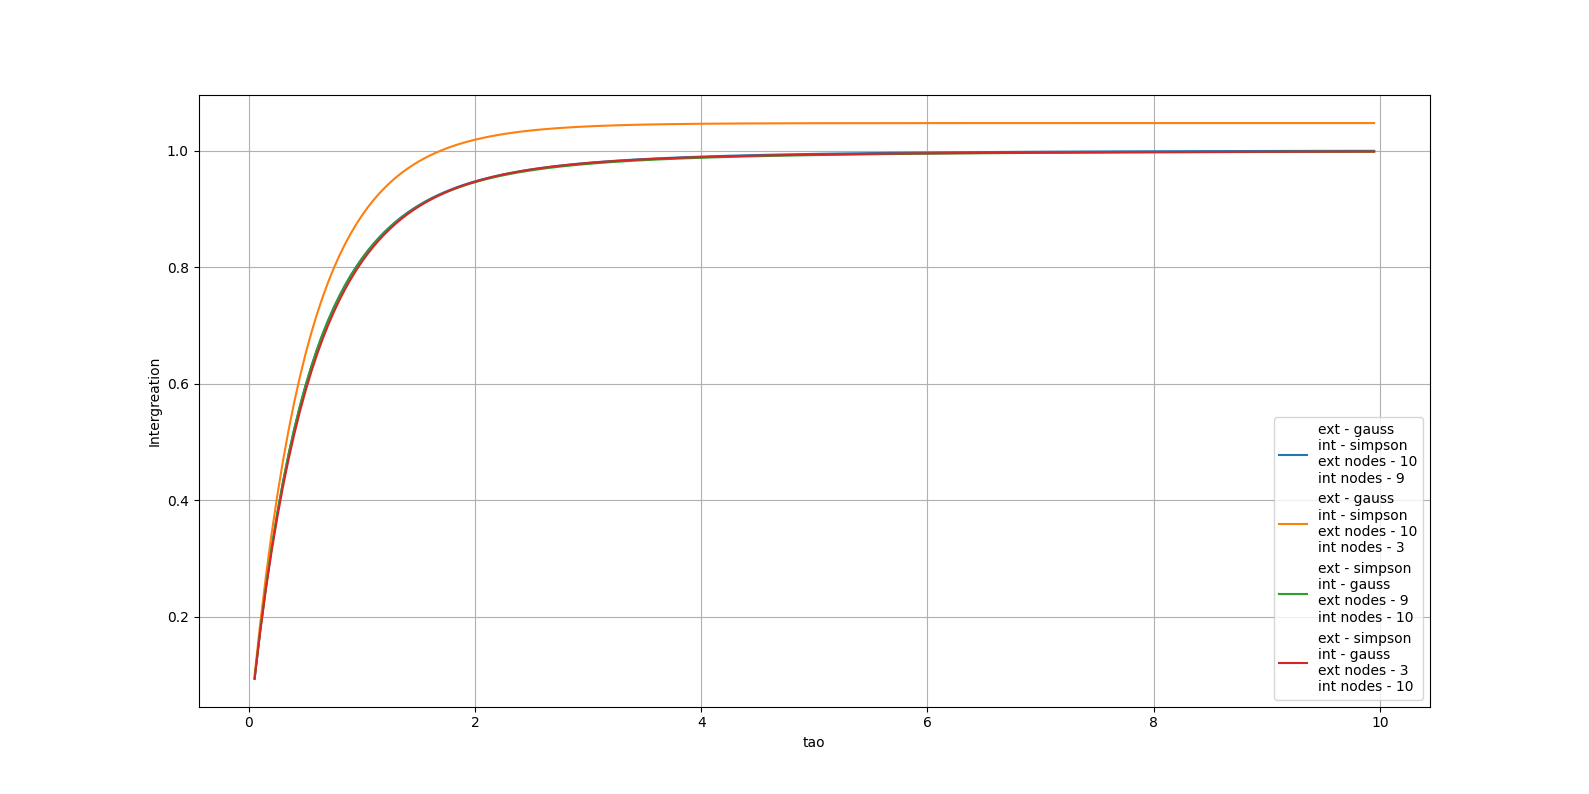
\includegraphics[scale=0.42]{./screens/1.png}
        \caption{Использование метода Симпсона с разным количеством узлов}
        \label{fig:my_label}
    \end{figure}

Из графика видно, что метод Симпсона работает не точно при малом количестве узлов. Особенно это заметно при вычислении внутреннего интеграла.

    \item Исследование метода Гаусса
    \begin{figure}[H]
        \centering
        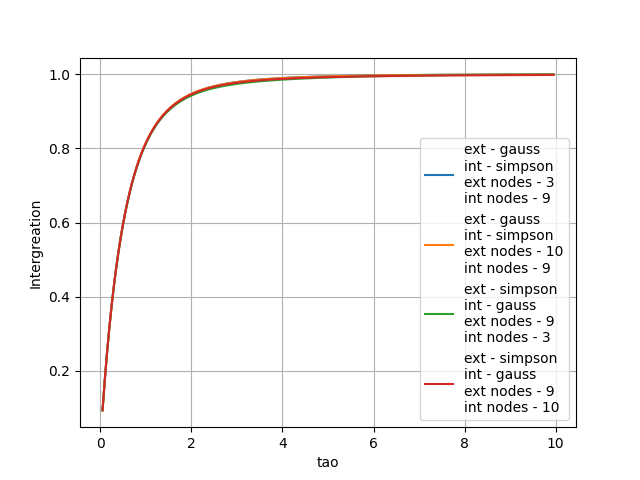
\includegraphics[scale=0.8]{./screens/2.png}
        \caption{Использование метода Гаусса с разным количеством узлов}
        \label{fig:my_label1}
    \end{figure}

Из графика видно, что метод Гаусса работает одинаково на разном количестве узлов.

    \item Построить график зависимости $\epsilon(\tau)$ диапазоне изменения $\tau = 0.05-10$. Указать при каком количестве узлов получены результаты.

см. пункт 2
\end{enumerate}



\section{Контрольные вопросы}
\subsection{В  каких  ситуациях  теоретический  порядок  квадратурных  формул  численного интегрирования не достигается.}
Если подинтегральная функция не имеет соответствующих производ-ных, то указанный теоретический порядок точности не достигается. Так, если на отрезке интегрирования не существуют 3-я и 4-я производные, то порядок точности формулы Симпсо-на будет только 2-ой

\subsection{Построить формулу Гаусса численного интегрирования при одном узле.}
Полином Лежандра 1 степени: \(P_1(x) = x\). Корень - $t_1 = 0$. Коэффициент $A_1 = 2$. Подставляем в формулу для вычисления интеграла и получаем:
\[\int_{a}^{b}f(x)dx = (b - a)f(\frac{b + a}{2})\]

\subsection{Построить формулу Гаусса численного интегрирования при двух узлах.}
Полином Лежандра 2 степени: \(P_2(x) = \frac{1}{2}(3x^2 - 1)\). Корни: $t_1 = \frac{1}{\sqrt{3}}$ и 
$t_2 = -\frac{1}{\sqrt{3}}$. Получим СЛАУ для вычисления коэффициентов:

\[
\begin{cases}
    A_1 + A_2 = 2 \\
    A_1 * \frac{1}{\sqrt{3}} - A_2 * \frac{1}{\sqrt{3}} = 0
\end{cases}
\]

Из СЛАУ получаем, что $A_1 = A_2 = 1$. Подставляем в формулу для вычисления интеграла и получаем:
\[\int_{a}^{b}f(x)dx = \frac{b - a}{2}(f(\frac{b + a}{2} - \frac{b - a}{2\sqrt{3}}) + f(\frac{b + a}{2} + \frac{b - a}{2\sqrt{3}}))\]

\subsection{Получить обобщенную кубатурную формулу, аналогичную  (6.6)  из лекции №6, для вычисления  двойного  интеграла  методом  последовательного  интегрированияна  основе формулы трапеций с тремяузлами по каждому направлению.}

\[\int_{c}^{d}\int_{a}^{b} f(x, y)dxdy = h_x(\frac{1}{2}(F_0 + F_2) + F_1)\]
Здесь,
\begin{align*}
    F_0 = h_y(\frac{1}{2}(f(x_0, y_0) + f(x_0, y_2)) + f(x_0, y_1))\\
    F_1 = h_y(\frac{1}{2}(f(x_1, y_0) + f(x_1, y_2)) + f(x_1, y_1))\\
    F_2 = h_y(\frac{1}{2}(f(x_2, y_0) + f(x_2, y_2)) + f(x_2, y_1))
\end{align*}

Подставим эти выражения в первую формулу:
\begin{multline*}
    \int_{c}^{d}\int_{a}^{b} f(x, y)dxdy = h_x(\frac{1}{2}(h_y(\frac{1}{2}(f(x_0, y_0) + f(x_0, y_2)) + f(x_0, y_1)) + \\h_y(\frac{1}{2}(f(x_2, y_0) + f(x_2, y_2)) + f(x_2, y_1))) + \\h_y(\frac{1}{2}(f(x_1, y_0) + f(x_1, y_2)) + f(x_1, y_1)))
\end{multline*}

\end{document}